\section{(5) Asynchronous communication models as classes of MSCs, MSO-definability}

\subsection{Definitions}

A Message Sequence Chart (MSC), such as the one in Fig.~\ref{}, provides a visual description of the behaviour of a distributed system. In this section, we start by formally defining the most generic class of Message Sequence Charts (MSCs), which we call asynchronous MSCs. More specialized classes of MSCs, such as $\pp$ MSCs, will also be discussed. Intuitively, we say that an MSC $\msc$ is asynchronous if there is an asynchronous system $\System$ that can exhibit the behaviour described by $\msc$. 

\begin{definition}[Asynchronous MSC]
An \emph{asynchronous MSC} (or simply MSC) over $\Procs$ and $\Msg$ is a tuple $\msc = (\Events,\procrel,\lhd,\lambda)$, where $\Events$ is a finite (possibly empty) set of \emph{events} and $\lambda: \Events \to \Act$ is a labeling function that associates an action to each event. For $p \in \Procs$, let $\Events_p = \{e \in \Events \mid \lambda(e) \in \pAct{p}\}$ be the set of events that are executed by $p$. We require that $\procrel$ (the \emph{process relation}) is the disjoint union $\bigcup_{p \in \Procs} \procrel_p$ of relations ${\procrel_p} \subseteq \Events_p \times \Events_p$ such that $\procrel_p$ is the direct successor relation of a total order on $\Events_p$. For an event $e \in \Events$, a set of actions $A \subseteq \Act$, and a relation $\rel \subseteq \Events \times \Events$,
let $\sametype{e}{A}{\rel} = |\{f \in \Events \mid (f,e) \in \rel$ and $\lambda(f) \in A\}|$. We require that ${\lhd} \subseteq \Events \times \Events$ (the \emph{message relation}) satisfies the following:
\begin{itemize}\itemsep=0.5ex
\item[(1)] for every pair $(e,f) \in {\lhd}$, there is a send action $\sact{p}{q}{\msg} \in \Act$ such that $\lambda(e) = \sact{p}{q}{\msg}$, $\lambda(f) = \ract{p}{q}{\msg}$.
\item[(2)] for all $f \in \Events$ such that $\lambda(f)$ is a receive action, there is exactly one $e \in \Events$ such that $e \lhd f$.
\end{itemize}
Finally, letting ${\le}_\msc = ({\procrel} \cup {\lhd})^\ast$,
we require that $\le_\msc$ is a partial order. For convenience, we simply write $\le$ when $M$ is clear from the context. We will refer to $\le$ as the \emph{causal ordering} or \emph{happens-before} relation. If, for two events $e$ and $f$, we have that $e \le f$, we will equivalently say that there is a \emph{causal path} between $e$ and $f$.
\end{definition}

According to Condition (2), every receive event must have a matching send event. Note that, however, there may be unmatched send events.
We let
$\SendEv{\msc} = \{e \in \Events \mid \lambda(e)$ is a send
action$\}$,
$\RecEv{\msc} = \{e \in \Events \mid \lambda(e)$ is a receive
action$\}$,
$\Matched{\msc} = \{e \in \Events \mid$ there is $f \in \Events$
such that $e \lhd f\}$, and
$\Unm{\msc} = \{e \in \Events \mid \lambda(e)$ is a send
action and there is no $f \in \Events$ such that $e \lhd f\}$.
%
We do not distinguish isomorphic MSCs and
let $\asMSCs$ be the set of all the asynchronous MSCs over the given sets $\Procs$ and $\Msg$.

% \paragraph*{Linearizations.}

% Consider $\msc = (\Events,\procrel,\lhd,\lambda) \in \asMSCs$.
% An \emph{asynchronous linearization} of $\msc$ is a (reflexive) total order ${\linrel} \subseteq \Events \times \Events$ such that ${\le_\msc} \subseteq {\linrel}$. Intuitively, an asynchronous linearization of $\msc$ is a possible ordering of its events.
% \davide{Example of asynchronous linearization.}

\paragraph*{Linearizations.}

Consider $\msc = (\Events,\procrel,\lhd,\lambda) \in \asMSCs$.
A \emph{linearization} of $\msc$ is a (reflexive) total order ${\linrel} \subseteq \Events \times \Events$ such that ${\le_\msc} \subseteq {\linrel}$. In other words, a linearization of $\msc$ is a total order that respects the happens-before relation $\le_\msc$ defined over $\msc$.
\davide{Provide example of linearization.}

\medskip

Asynchronous MSCs are the widest class of MSCs that we will deal with. By introducing additional constraints, we are able to define other classes of MSCs that exclusively describe the behaviours of \pp systems, mailbox systems, and so on.
\davide{Provide example of asynchronous MSC that is not p2p.}

As in the asynchronous case, we say that $\msc$ is a \pp MSC if there is a \pp system that can produce the behaviour described by $\msc$. We give here the formal definition of \pp MSC, which also considers the possibility of having unmatched messages (i.e. messages that are sent but not received).
\davideanswer{Why unmatched messages? What do they represent? When an automata does not have the receive action for a message that was already sent (see examples at the end of concur paper).}

\begin{definition}[Peer-to-peer MSCs]
A \emph{\pp MSC} (or simply \emph{MSC}) is an asynchronous MSC where we require that, for every pair $(e,f) \in {\lhd}$, such that $\lambda(e) = \sact{p}{q}{\msg}$, $\lambda(f) = \ract{p}{q}{\msg}$, we have $\sametype{e}{\pqsAct{p}{q}}{\procrel^+} = \sametype{f}{\pqrAct{p}{q}}{\procrel^+}$.
\end{definition}

The additional constraint satisfied by \pp MSCs ensures that channels operate in FIFO mode; when a process $q$ receives a message from a process $p$, it must have already received all the messages that were previously sent to him by $p$. Let $\ppMSCs$ denote the set of all the \pp MSCs over two given sets $\Procs$ and $\Msg$. Note that, by definition, every \pp MSC is an asynchronous MSC. The idea is that we are always able to find an asynchronous system that \emph{can} exhibit the behaviour described by a \pp MSC; after all, the channels of an asynchronous system do not have to follow any specific behaviour, so they can indeed happen to operate as if they were queues. Example~\ref{} shows that the opposite direction is generally not true, an asynchronous MSC is not always a \pp MSC. It follows that $\ppMSCs \subset \asMSCs$.

\medskip

We will now consider the class of MSCs for which there is a causally ordered system that can produce their behaviour. Intuitively, an MSC is causally ordered if all the messages sent to the same process are received in an order which is consistent with the causal ordering of the corresponding send events. Below the formal definition, which also considers unmatched messages.
\davide{Provide example of an MSC that is not causally ordered}
\begin{definition}[Causally ordered MSC]
An MSC $\msc = (\Events,\procrel,\lhd,\lambda)$ is \emph{causally ordered} if, for any two send events $s$ and $s'$, such that $\lambda(s)=\pqsAct{\plh}{q}$, $\lambda(s')=\pqsAct{\plh}{q}$, and $s \le_\msc s'$, we have either:
\begin{itemize}\itemsep=0.5ex
	\item $s,s' \in \Matched{\msc}$ and $r \procrel^* r'$, where $r$ and $r'$ are two receive events such that $s \lhd r$ and $s' \lhd r'$.
	\item $s' \in \Unm{\msc}$.
\end{itemize}
\end{definition}

By definition, every causally ordered MSC is a \pp MSC. This is not surprising, considering that a causally ordered system is essentially a \pp system with an additional constraint on the delivery of messages; indeed, we are always able to find a \pp system that \emph{can} exhibit the behaviour described by a causally ordered MSC. Let $\coMSCs$ denote the set of all the causally ordered MSCs over two given sets $\Procs$ and $\Msg$. Example~\ref{} shows that a \pp MSC is not always a causally ordered MSC. It follows that $\coMSCs \subset \ppMSCs$.

\medskip

Moving on to the mailbox semantics, we say that $\msc$ is a mailbox MSC if there is a mailbox system that can exhibit the behaviour described by $\msc$. 
\davide{Provide example of MSC which is not mailbox}

\begin{definition}[Mailbox MSC]\label{def:mb_msc}
An MSC $\msc = (\Events,\procrel,\lhd,\lambda)$ is a \emph{mailbox MSC} if it has a linearization $\linrel$ where, for any two send events $s$ and $s'$, such that $\lambda(s)=\pqsAct{\plh}{q}$, $\lambda(s')=\pqsAct{\plh}{q}$, and $s \linrel s'$, we have either:
\begin{itemize}\itemsep=0.5ex
	\item $s,s' \in \Matched{\msc}$ and $r \linrel r'$, where $r$ and $r'$ are two receive events such that $s \lhd r$ and $s' \lhd r'$.
	\item $s' \in \Unm{\msc}$.
\end{itemize}
\end{definition}

Such a linearization will be referred to as a \emph{mailbox linearization}, and the symbol $\mblinrel$ will be used to denote one. Let $\mbMSCs$ denote the set of all the mailbox MSCs over two given sets $\Procs$ and $\Msg$. By definition, every mailbox MSC is a \pp MSC. Conversely, Example~\ref{} shows a \pp MSC which is not a mailbox MSC. It follows that $\mbMSCs \subset \ppMSCs$. We show here that each mailbox MSC is also a causally ordered MSC.
\davide{Provide example of causally ordered MSC which is not mailbox (Figure 2.18 of Laetitia's thesis).}

\begin{proposition}\label{prop:mb_is_co}
	Every mailbox MSC is a causally ordered MSC.
\end{proposition}
\begin{proof}
Let $\msc$ be a mailbox MSC and $\linrel$ a mailbox linearization of it. Recall that a linearization has to respect the happens-before partial order over $\msc$, i.e. $\le_\msc \,\subseteq\, \linrel$. Consider any two send events $s$ and $s'$, such that $\lambda(s)=\pqsAct{\plh}{q}$, $\lambda(s')=\pqsAct{\plh}{q}$ and $s \le_\msc s'$. Since $\le_\msc \,\subseteq\, \linrel$, we have that $s \linrel s'$ and, by the definition of mailbox linearization, either
\begin{enumerate*}[label={(\roman*)}]
	\item $s' \in \Unm{\msc}$, or 
	\item $s,s' \in \Matched{\msc}$, $s \lhd r$, $s' \lhd r'$ and $r \linrel r'$. 
\end{enumerate*}
The former clearly respects the definition of causally ordered MSC, so let us focus on the latter. Note that $r$ and $r'$ are two receive events executed by the same process, hence $r \linrel r'$ implies $r \procrel^+ r'$. It follows that $\msc$ is a causally ordered MSC.
\end{proof}

\medskip

Moving on to the $\onen$ semantics, we say that $\msc$ is a $\onen$ MSC if there is a $\onen$ system that can exhibit the behaviour described by $\msc$. 

\begin{definition}[$\onen$ MSC]\label{def:one_n}
An MSC $\msc = (\Events,\procrel,\lhd,\lambda)$ is a \emph{$\onen$ MSC} if it has a linearization $\linrel$ where, for any two send events $s$ and $s'$, such that $\lambda(s)=\pqsAct{p}{\plh}$, $\lambda(s')=\pqsAct{p}{\plh}$, and $s \procrel^+ s'$ (which implies $s \linrel s'$), we have either:
\begin{itemize}\itemsep=0.5ex
	\item $s,s' \in \Matched{\msc}$ and $r \linrel r'$, where $r$ and $r'$ are two receive events such that $s \lhd r$ and $s' \lhd r'$.
	\item $s' \in \Unm{\msc}$.
\end{itemize}
\end{definition}

Such a linearization will be referred to as a \emph{$\onen$ linearization}. Note that the definition is very similar to the mailbox case, but here $s$ and $s'$ are two send events executed by the same process. Let $\onenMSCs$ denote the set of all the $\onen$ MSCs over two given sets $\Procs$ and $\Msg$. By definition, every $\onen$ MSC is a \pp MSC. Conversely, Example~\ref{} shows a \pp MSC which is not a $\onen$ MSC. It follows that $\mbMSCs \subset \ppMSCs$. We show here that each $\onen$ MSC is also a causally ordered MSC, which is not as intuitive as the mailbox case.

\davide{Provide example of MSC which is not $\onen$}

\davidequestion{Should I still leave this proof if we showed that every $\onen$ MSC is a mailbox MSC?}
\begin{proposition}\label{prop:onen_is_co}
	Every $\onen$ MSC is a causally ordered MSC.
\end{proposition}
\begin{proof}
By contradiction. Suppose that $\msc$ is a $\onen$ MSC, but not a causally ordered MSC. Since $\msc$ is not causally ordered, there must be two send events $s$ and $s'$ such that $\lambda(s)=\pqsAct{\plh}{q}$, $\lambda(s')=\pqsAct{\plh}{q}$, $s \le_\msc s'$, and we have either:
\begin{enumerate}\itemsep=0.5ex
	\item $s,s' \in \Matched{\msc}$ and $r' \procrel^* r$, where $r$ and $r'$ are two receive events such that $s \lhd r$ and $s' \lhd r'$.
	\item  $s \in \Unm{\msc}$ and $s' \in \Matched{\msc}$.
\end{enumerate}
We need to show that both of these scenarios lead to a contradiction. (1) Suppose $s$ and $s'$ are executed by the same process. Since $\msc$ is a $\onen$ MSC, there must be a linearization $\linrel$ such that $r \linrel r'$, but this is clearly impossible since we have $r' \procrel^* r$. Suppose now that $s$ and $s'$ are executed by two different processes $p$ and $q$. We know by hypothesis that $s \le_\msc s'$, i.e. there is a causal path of events $P = s \sim a \sim \dots \sim s' \sim r'$ from $s$ to $r'$, where $\sim$ is either $\procrel$ or $\lhd$. Refer to the first example in Figure~\ref{fig:onen_is_co} for a visual representation ($P$ is drawn in purple). To have a causal path $P$, there must be a send event $s''$ that is executed by $p$ after $s$ and that is part of $P$, along with its receipt $r''$ (i.e. $P = s \le_\msc s'' \lhd r'' \le_\msc s' \lhd r'$). We clearly have $r'' \linrel r'$ for any linearization of $\msc$, because $r'' \le_\msc r'$ (they are both in the causal path $P$ and $r''$ happens before $r$). Since $\msc$ is a $\onen$ MSC, there has to be a linearization $\linrel$ where $r \linrel r''$, because $s$ and $s''$ are send events executed by the same process. It follows that $\msc$ should have a linearization were $r \linrel r'' \linrel r'$, but this is not possible because of the hypothesis that $r' \procrel^* r$. This is a contradiction. (2) Suppose $s$ and $s'$ are executed by the same process. It is trivial to see, by definition, that $\msc$ cannot be a $\onen$ MSC. Suppose now that $s$ and $s'$ are executed by two different processes $p$ and $q$, and consider the same send event $s''$ as before (executed by $p$). Refer to the second example in Figure~\ref{fig:onen_is_co} for a visual representation. Since $s''$ is matched, we have two events $s$ and $s''$, sent by the same process $p$, that are unmatched and matched, respectively. Clearly, $\msc$ cannot be a $\onen$ MSC.
\end{proof}

\begin{figure}[h]
	\centering
	\begin{subfigure}[b]{0.4\textwidth}
		\begin{center}
			\begin{tikzpicture}
				\newproc{0}{p}{-2.1};
				\newproc{1}{t}{-2.1};
				\newproc{2}{q}{-2.1};
			
				% \newmsgdiagnoname{0}{1}{-0.2}{-2.5}{black};
				\newmsgnoname{0}{1}{-0.3}{black};
				\newmsgnoname{0}{2}{-1}{black};
				\newmsgnoname{2}{1}{-1.7}{black};
		
				\newevent{black}{0}{-0.3}{s}{left};
				\newevent{black}{0}{-1}{s''}{left};
				\newevent{black}{2}{-1}{r''}{above right};
				\newevent{black}{1}{-1.7}{r'}{above right};
				\newevent{black}{2}{-1.7}{s'}{right};
				\newevent{black}{1}{-0.3}{r}{right};
		
				\newflechevert{Purple}{0}{-0.3}{-1};
				\newflechehor{Purple}{-1}{0}{2};
				\newflechevert{Purple}{2}{-1}{-1.7};
				\newflechehorinverse{Purple}{-1.7}{2}{1};
				
			\end{tikzpicture}
		\end{center}
	\end{subfigure}
	% \hfill
	\begin{subfigure}[b]{0.4\textwidth}
		\begin{center}
			\begin{tikzpicture}
				\newproc{0}{p}{-2.1};
				\newproc{1}{t}{-2.1};
				\newproc{2}{q}{-2.1};
			
				% \newmsgdiagnoname{0}{1}{-0.2}{-2.5}{black};
				\newmsgumnoname{0}{1}{-0.3}{black};
				\newmsgnoname{0}{2}{-1}{black};
				\newmsgnoname{2}{1}{-1.7}{black};
		
				\newevent{black}{0}{-0.3}{s}{left};
				\newevent{black}{0}{-1}{s''}{left};
				\newevent{black}{2}{-1}{r''}{above right};
				\newevent{black}{2}{-1.7}{s'}{right};
				\newevent{black}{1}{-1.7}{r'}{above right};
		
				\newflechevert{Purple}{0}{-0.3}{-1};
				\newflechehor{Purple}{-1}{0}{2};
				\newflechevert{Purple}{2}{-1}{-1.7};
				\newflechehorinverse{Purple}{-1.7}{2}{1};
				
			\end{tikzpicture}
			\end{center}
	\end{subfigure}
	   \caption{Two examples of $\onen$ MSCs.}
	   \label{fig:onen_is_co}
\end{figure}

\davide{Provide example of causally ordered MSC which is not $\onen$ (same as mailbox! Figure 2.18 of Laetitia's thesis).}

\begin{definition} [$\onen$ alternative]\label{def:one_n_alt}
For an MSC $\msc = (\Events,\procrel,\lhd,\lambda)$, we define
an additional binary relation that represents a constraint
under the $\onen$ semantics, which ensures that messages sent from the same process are received in the same order. Let ${\onenrel}_\msc \subseteq \Events \times \Events$ be defined as $e_1 \onenrel_\msc e_2$ if there are two events $e_1$ and $e_2$, and $p \in \Procs$ such that either:
\begin{itemize}\itemsep=0.5ex
	\item $\lambda(e_1) \in \psAct{p}$, $\lambda(e_2) \in \psAct{p}$, $e_1 \in \Matched{\msc}$, and $e_2 \in \Unm{\msc}$, or
	\item $\lambda(e_1) \in \prAct{p}$, $\lambda(e_2) \in \prAct{p}$, $s_1 \lhd e_1$ and $s_2 \lhd e_2$ for some $s_1,s_2 \in \Events_p$, and $s_1 \procrel^+ s_2$.
\end{itemize}

We let ${\lessdot_\msc} = ({\procrel} \,\cup\, {\lhd} \,\cup\, {\onenrel_\msc})^\ast$.
Note that ${\le_\msc} \subseteq {\lessdot_\msc}$.
%
%\begin{definition}\label{def:mailbox-msc}
	We call $\msc \in \asMSCs$ a \emph{$\onen$ MSC}
	if ${\lessdot_\msc}$ is a partial order.
\end{definition}

\davidequestion{Should I also include the proof that every mailbox MSC without unmatched messages is $\onen$? Do we need it?}

\begin{proposition}\label{prop:onen_mb_no_unmatched}
	Every $\onen$ MSC without unmatched messages is a mailbox MSC.
\end{proposition}
\begin{proof}
We show that the contrapositive is true, i.e. if an MSC is not mailbox (and it does not have unmatched messages), it is also not $\onen$. Suppose $\msc$ is an asynchronous MSC, but not mailbox. There must be a cycle $\xi$ such that  $e \preceq e$, for some event $e$. Recall that ${\preceq} = ({\procrel} \,\cup\, {\lhd} \,\cup\, {\mbrel})^\ast$ and ${\le} = ({\procrel} \cup {\lhd})^\ast$. We can always explicitely write a cycle $e \preceq e$ only using $\mbrel$ and $\le$. For instance, there might be a cycle $e \preceq e$ because we have that $e \mbrel f \le g \mbrel h \mbrel i \le e$. Consider any two adiacent events $s_1$ and $s_2$ in the cycle $\xi$, where $\xi$ has been written using only $\mbrel$ and $\le$, and we never have two consecutive $\le$\footnote{This is always possible, since $a \le b \le c$ is written as $a \le c$.}. We have two cases:
\begin{enumerate}
	\item $s_1 \mbrel s_2$. We know, by definition of $\mbrel$, that $s_1$ and $s_2$ must be two send events and that $r_1 \procrel^+ r_2$, where $r_1$ and $r_2$ are the receive events that match with $s_1$ and $s_2$, respectively (we are not considering unmatched messages by hypothesis).
	\item $s_1 \le s_2$. Since $\msc$ is asynchronous by hyphotesis, $\xi$ has to contain at least one $\mbrel$\footnote{If that was not the case, $\le$ would also be cyclic and $\msc$ would not be an asynchronous MSC.}; recall that we also wrote $\xi$ in such a way that we do not have two consecutive $\le$. It is not difficult to see that $s_1$ and $s_2$ have to be send events, since they belong to $\xi$. We have two cases:
	\begin{enumerate}
		\item $r_1$ is in the causal path, i.e. $s_1 \lhd r_1 \le s_2$. In particular, note that $r_1 \le r_2$.
		\item $r_1$ is not in the causal path, hence there must be a message $m_k$ sent by the same process that sent $s_1$, such that $s_1 \procrel^+ s_k \lhd r_k \le s_2 \lhd r_2$, where $s_k$ and $r_k$ are the send and receive events associated with $m_k$, respectively. Since messages $m_1$ and $m_k$ are sent by the same process and $s_1 \procrel^+ s_k$, we should have $r_1 \onenrel r_k$, according to the $\onen$ semantics. In particular, note the we have $r_1 \onenrel r_k \le r_2$.
	\end{enumerate}
	In both case (a) and (b), we conclude that $r_1 \lessdot r_2$. Recall that ${\lessdot} = ({\procrel} \,\cup\, {\lhd} \,\cup\, {\onenrel_\msc})^\ast$.
\end{enumerate}
Notice that, for either cases, a relation between two send events $s_1$ and $s_2$ (i.e. $s_1 \mbrel s_2$ or $s_1 \le s_2$) always implies a relation between the respective receive events $r_1$ and $r_2$, according to the $\onen$ semantics. It follows that $\xi$, which is a cycle for the $\preceq$ relation, always implies a cycle for the $\lessdot$ relation\footnote{If $\lessdot$ is cyclic, $\msc$ is not a $\onen$ MSC.}, as shown by the following example. Let $\msc$ be a non-mailbox MSC, and suppose we have a cycle $s_1 \mbrel s_2 \mbrel s_3 \le s_4 \mbrel s_5 \le s_1$. $s_1 \mbrel s_2$ falls into case (1), so it implies $r_1 \procrel^+ r_2$. The same goes for $s_2 \mbrel r_3$, which implies $r_2 \procrel^+ r_3$. $s_3 \le s_4$ falls into case (2), and implies that $r_3 \lessdot r_4$. $s_4 \mbrel s_5$ falls into case (1) and it implies $r_4 \procrel^+ r_5$. $s_5 \le s_1$ falls into case (2) and implies that $r_5 \lessdot r_1$. Putting all these implications together, we have that $r_1 \procrel^+ r_2 \procrel^+ r_3 \lessdot r_4 \procrel^+ r_5 \lessdot r_1$, which is a cycle for $\lessdot$. Note that, given any cycle for $\preceq$, we are always able to apply this technique to obtain a cycle for $\lessdot$.
\end{proof}

Proposition~\ref{prop:onen_mb_no_unmatched} remains true even if we consider unmatched messages.

\begin{proposition}\label{prop:onen_mb_unmatched}
	Every $\onen$ MSC is a mailbox MSC.
\end{proposition}
\begin{proof}
Let $\msc$ be an asynchronous MSC. The proof proceeds in the same way as the one of Proposition~\ref{prop:onen_mb_no_unmatched}, but unmatched messages introduce some additional cases. Consider any two adiacent events $s_1$ and $s_2$ in a cycle $\xi$ for $\preceq$, where $\xi$ has been written using only $\mbrel$ and $\le$, and we never have two consecutive $\le$. These are some additional cases:
\begin{enumerate}\setcounter{enumi}{2}
	\item $u_1 \mbrel s_2$, where $u_1$ is the send event of an unmatched message. This case never happens because of how $\mbrel$ is defined.
	\item $u_1 \le u_2$, where $u_1$ and $u_2$ are both send events of unmatched messages. Since both $u_1$ and $u_2$ are part of the cycle $\xi$, there must be an event $s_3$ such that $u_1 \le u_2 \mbrel s_3$. However, $u_2 \mbrel s_3$ falls into case (3), which can never happen.
	\item $u_1 \le s_2$, where $u_1$ is the send event of an unmatched message and $s_2$ is the send event of a matched message. Since we have a causal path between $u_1$ and $s_2$, there has to be a message $m_k$, sent by the same process that sent $m_1$, such that $u_1 \procrel^+ s_k \lhd r_k \le s_2 \lhd r_2$\footnote{Note that we can have $m_k = m_2$}, where $s_k$ and $r_k$ are the send and receive events associated with $m_k$, respectively. Since messages $m_1$ and $m_k$ are sent by the same process and $m_1$ is unmatched, we should have $s_k \onenrel u_1$, according to the $\onen$ semantics, but $u_1 \procrel^+ s_k$. It follows that if $\xi$ contains $u_1 \le s_2$, we can immediately conclude that $\msc$ is not a $\onen$ MSC.
	\item $s_1 \mbrel u_2$,  where $s_1$ is the send event of a matched message and $u_2$ is the send event of an unmatched message. Since both $s_1$ and $u_2$ are part of a cycle, there must be an event $s_3$ such that $s_1 \mbrel u_2 \le s_3$; we cannot have $u_2 \mbrel s_3$, because of case (3). $u_2 \le s_3$ falls into case (5), so we can conclude that $\msc$ is not a $\onen$ MSC.
\end{enumerate}
We showed that cases (3) and (4) can never happen, whereas cases (5) and (6) both imply that $\msc$ is not $\onen$. If we combine them with the cases described in Proposition~\ref{prop:onen_mb_no_unmatched} we have the full proof.
\end{proof}

\begin{definition}[$\nn$ MSC]\label{def:n_n}
	An MSC $\msc = (\Events,\procrel,\lhd,\lambda)$ is a \emph{$\nn$ MSC} if it has a linearization $\linrel$ where, for any two send events $s$ and $s'$, such that $s \linrel s'$, we have either:
	\begin{itemize}\itemsep=0.5ex
		\item $s,s' \in \Matched{\msc}$ and $r \linrel r'$, where $r$ and $r'$ are two receive events such that $s \lhd r$ and $s' \lhd r'$.
		\item $s' \in \Unm{\msc}$.
	\end{itemize}
\end{definition}

Such a linearization will be referred to as a \emph{$\nn$ linearization}. Intuitively, with an $\nn$ MSC we are always able to schedule events in such a way that messages are received in the same order as they were sent, and unmatched messages are sent only after all matched messages are sent. By definition, every $\nn$ MSC is a $\onen$ MSC. 

\begin{definition} [$\nn$ alternative]\label{def:n_n_alt}
For an MSC $\msc = (\Events,\procrel,\lhd,\lambda)$, let ${\nnrel}_\msc = ({\procrel} \,\cup\, {\lhd} \,\cup\, {\mbrel_\msc} \,\cup\, {\onenrel_\msc})^\ast$. We define an additional binary relation $\bowtie_\msc \subseteq \Events \times \Events$, such that for two events $e_1$ and $e_2$ we have $e_1 \bowtie_\msc e_2$ if one of the following holds:
\begin{enumerate}\itemsep=0.5ex
	\item $e_1 \nnrel_\msc e_2$
	\item $\lambda(e_1) \in \prAct{\plh}$, $\lambda(e_2) \in \prAct{\plh}$, $s_1 \lhd e_1$ and $s_2 \lhd e_2$ for some $s_1,s_2 \in \Events$, $s_1 \nnrel_\msc s_2$ and $e_1 \slashed{\nnrel}_\msc e_2$.
	\item $\lambda(e_1) \in \psAct{\plh}$, $\lambda(e_2) \in \psAct{\plh}$, $e_1 \lhd r_1$ and $e_2 \lhd r_2$ for some $r_1,r_2 \in \Events$, $r_1 \nnrel_\msc r_2$ and $e_1 \slashed{\nnrel}_\msc e_2$.
	\item $e_1 \in \Matched{\msc}$, $e_2 \in \Unm{\msc}$, $e_1 \slashed{\nnrel}_\msc e_2$.
\end{enumerate}

Note that $\preceq_\msc \subseteq \nnrel_\msc$, $\lessdot_\msc \subseteq \nnrel_\msc$, and $\nnrel_\msc \subseteq\; \bowtie_\msc$. We call $\msc \in \asMSCs$ a \emph{$\nn$ MSC}
if ${\bowtie_\msc}$ is acyclic.
\davidequestion{Initially I said "We call $\msc \in \asMSCs$ a \emph{$\nn$ MSC} if ${\bowtie_\msc}$ is a partial order", but I don't think it is true, since $\bowtie_\msc$ does not have to be transitive.}
\end{definition}

It is not trivial to see that Definition~\ref{def:n_n_alt} is equivalent to Definition~\ref{def:n_n}. To show that, we need some preliminary results and definitions. 

\begin{proposition}
	Let $\msc$ be an MSC. Given two matched send events $s_1$ and $s_2$, and their respective receive events $r_1$ and $r_2$, $r_1 \bowtie_\msc r_2 \implies s_1 \bowtie_\msc s_2$.
\end{proposition}
\begin{proof}
Follows from the definition of $\bowtie_\msc$. We have $r_1 \bowtie_\msc r_2$ if either:
\begin{itemize}\itemsep=0.5ex
	\item $r_1 \nnrel_\msc r_2$. Two cases: either \begin{enumerate*}[label={(\roman*)}]
		\item $s_1 \nnrel_\msc s_2$, or 
		\item $s_1 \slashed{\nnrel}_\msc s_2$.
	\end{enumerate*}
	The first case clearly implies $s_1 \bowtie_\msc s_2$, for rule 1 in the definition of $\bowtie_\msc$. The second too, because of rule 3.
	\item  $r_1 \slashed{\nnrel}_\msc r_2$, but $r_1 \bowtie_\msc r_2$. This is only possible if rule 2 in the definition of $\bowtie_\msc$ was used, which implies $s_1 \nnrel_\msc s_2$ and, for rule 1, $s_1 \bowtie_\msc s_2$.
\end{itemize}
\end{proof}

\begin{proposition}\label{prop:n_n_cycl}
	Let $\msc$ be an MSC. If $\bowtie_\msc$ is cyclic, then $\msc$ is not $\nn$.
\end{proposition}
\begin{proof}
Since a $\nn$ MSC is always both a mailbox and a $\onen$ MSC, it is clear that the cyclicity of $\nnrel_\msc$ implies that $\msc$ is not $\nn$, because it means that we are not even able to find a linearization that is both mailbox and $\onen$. Moreover, since in a $\nn$ linearization the order in which messages are sent matches the order in which they are received, and unmatched send events can be executed only after matched send events, a $\nn$ MSC always has to satisfy the constraints imposed by the $\bowtie_\msc$ relation. If $\bowtie_\msc$, then for sure there is no $\nn$ linearization for $\msc$.
\end{proof}

Let the \emph{Event Dependency Graph} (EDG) of a $\nn$ MSC $\msc$ be a graph that has events as nodes and an edge between two events $e_1$ and $e_2$ if $e_1 \bowtie_\msc e_2$. We now present an algorithm that, given the EDG of an $\nn$ MSC $\msc$, computes a $\nn$ linearization of $\msc$. We then show that, if $\bowtie_\msc$ is acyclic (i.e. it is a partial order), this algorithm always terminates correctly. This, along with Proposition~\ref{prop:n_n_cycl}, effectively shows that Definition~\ref{def:n_n} and Definition~\ref{def:n_n_alt} are equivalent.

\paragraph*{Algorithm for finding a $\nn$ linearization}
The input of this algorithm is the EDG of an MSC $\msc$, and it outputs a valid $\nn$ linearization for $\msc$, if $\msc$ is $\nn$. The algorithm works as follows:
\begin{enumerate}
	\item If there is a matched send event $s$ with in-degree 0 in the EDG, add $s$ to the linearization and remove it from the EDG, along with its outgoing edges, then jump to step 5. Otherwise, proceed to step 2.
	\item If there are no matched send events in the EDG and there is an unmatched send event $s$ with in-degree 0 in the EDG, add $s$ to the linearization and remove it from the EDG, along with its outgoing edges, then jump to step 5. Otherwise, proceed to step 3.
 	\item If there is a receive event $r$ with in-degree 0 in the EDG, such that $r$ is the receive event of the first message whose sent event was already added to the linearization, add $r$ to the linearization and remove it from the EDG, along with its outgoing edges, then jump to step 5. Otherwise, proceed to step 4.
   	\item Throw an error and terminate.
   	\item If all the events of $\msc$ were added to the linearization, return the linearization and terminate. Otherwise, go back to step 1.
\end{enumerate} 

We now need to show that 
\begin{enumerate*}[label={(\roman*)}]
	\item if this algorithm terminates correctly (i.e. step 4 is never executed), it returns a $\nn$ linearization, and 
	\item if $\bowtie_\msc$ is acyclic, the algorithm always terminates correctly.
\end{enumerate*}
\begin{proposition}
	If the above algorithm returns a linearization for an MSC $\msc$, it is a $\nn$ linearization.
\end{proposition}
\begin{proof}
	Note that, because of how step 2 works, the order (in the linearization) in which matched messages are sent is the same as the order in which they are received. Moreover, according to step 3, an unmatched send events is added to the linearization only if all the matched send events were already added.
\end{proof}

\begin{proposition}
	Given an MSC $\msc$, the above algorithm always terminates correctly if $\bowtie_\msc$ is acyclic.
\end{proposition}
\begin{proof}
We want to prove that, if $\bowtie_\msc$ is acyclic, step 4 of the algorithm is never executed, i.e. it terminates correctly. Note that the acyclicity of $\bowtie_\msc$ implies that the EDG of $\msc$ is a DAG. Moreover, at every step of the algorithm we remove nodes and edges from the EDG, so it still remains a DAG. The proof goes by induction on the number of events added to the linearization.\newline
Base case: no event has been added to the linearization yet. Since the EDG is a DAG, there must be an event with in-degree 0. In particular, this has to be a send event (a receive event depends on its respective send event, so it cannot have in-degree 0). If it is a matched send event, step 1 is applied. If there are no matched send events, step 2 is applied on an unmatched send. We show that it is impossible to have an unmatched send event of in-degree 0 if there are still matched send events in the EDG, so either step 1 or 2 are applied in the base case. Let $s$ be one of those matched send events and let $u$ be an unmatched send. Because of rule 4 in the definition of $\bowtie_\msc$, we have that $s \bowtie_\msc u$, which implies that $u$ cannot have in-degree 0 if $s$ is still in the EDG.\newline
Inductive step: we want to show that we are never going to execute step 4. In particular, Step 4 is executed when none of the first three steps can be applied. This happens when there are no matched send events with in-degree 0 and one of the following holds:
\begin{itemize}\itemsep=0.5ex
	\item \emph{There are still matched send events in the EDG with in-degree $>0$, there are no unmatched messages with in-degree 0, and there is no receive event $r$ with in-degree 0 in the EDG, such that $r$ is the receive event of the first message whose sent event was already added to the linearization}. Since the EDG is a DAG, there must be at least one receive event with in-degree 0. We want to show that, between these receive events with in-degree 0, there is also the receive event $r$ of the first message whose send event was added to the linearization, so that we can apply step 3 and step 4 is not executed. Suppose, by contradiction, that $r$ has in-degree $>0$, so it depends on other events. For any maximal chain in the EDG that contains one of these events, consider the first event $e$, which clearly has in-degree 0. In particular, $e$ cannot be a send event, because we would have applied step 1 or step 2. Hence, $e$ can only be a receive event for a send event that was not the first added to the linearization (and whose respective receive still has not been added). However, this is also impossible, since $r_e \bowtie_\msc r$ implies $s_e \bowtie_\msc s$, and we could not have added $s$ to the linearization before $s_e$. Because we got to a contradiction, the hypothesis that $r$ has in-degree $>0$ must be false, and we can indeed apply step 3.
	\item \emph{There are still matched send events in the EDG with in-degree $>0$, there is at least one unmatched message with in-degree 0, and there is no receive event $r$ with in-degree 0 in the EDG, such that $r$ is the receive event of the first message whose sent event was already added to the linearization}. We show that it is impossible to have an unmatched send event of in-degree 0 if there are still matched send events in the EDG. Let $s$ be one of those matched send events and let $u$ be an unmatched send. Because of rule 4 in the definition of $\bowtie_\msc$, we have that $s \bowtie_\msc u$, which implies that $u$ cannot have in-degree 0 if $s$ is still in the EDG.
	\item \emph{There are no more matched send events in the EDG, there are no unmatched messages with in-degree 0, and there is no receive event $r$ with in-degree 0 in the EDG, such that $r$ is the receive event of the first message whose sent event was already added to the linearization}. Very similar to the first case. Since the EDG is a DAG, there must be at least one receive event with in-degree 0. We want to show that, between these receive events with in-degree 0, there is also the receive event $r$ of the first message whose send event was added to the linearization, so that we can apply step 3 and step 4 is not executed. Suppose, by contradiction, that $r$ has in-degree $>0$, so it depends on other events. For any maximal chain in the EDG that contains one of these events, consider the first event $e$, which clearly has in-degree 0. In particular, $e$ cannot be a send event, because by hypothesis there are no more send events with in-degree 0 in the EDG. Hence, $e$ can only be a receive event for a send event that was not the first added to the linearization (and whose respective receive still has not been added). However, this is also impossible, since $r_e \bowtie_\msc r$ implies $s_e \bowtie_\msc s$, and we could not have added $s$ to the linearization before $s_e$. Because we got to a contradiction, the hypothesis that $r$ has in-degree $>0$ must be false, and we can indeed apply step 3.
\end{itemize}
We showed that, if $\bowtie_\msc$ is acyclic, the algorithm always terminates correctly and computes a valid $\nn$ linearization.
\end{proof}

\begin{definition}[$\rsc$ MSC]\label{def:rsc}
	An MSC $\msc = (\Events,\procrel,\lhd,\lambda)$ is a \emph{RSC MSC} if it has no unmatched send events and there is a linearization $\linrel$ where any matched send event is immediately followed by its respective receive event.
\end{definition}

Following the characterization given in \cite[Theorem 4.4]{DBLP:journals/dc/Charron-BostMT96}, we also give an alternative but equivalent definition of $\rsc$ MSC.

\begin{definition}
	Let $\msc$ be an MSC. A crown of size $k$ in $\msc$ is a sequence $\langle(s_i,r_i),\, i \in \{1,\dots,k\}\rangle$ of pairs of corresponding send and receive events such that
	\[
		s_1 <_\msc r_2, s_2 <_\msc r_3, \dots, s_{k-1} <_\msc r_k, s_k <_\msc r_1.
	\]
\end{definition}
\davide{Specify somewhere that $<_\msc = (\procrel \cup \lhd)^+$.}

\begin{definition} [$\rsc$ alternative]\label{def:rsc_alt}
	An MSC $\msc = (\Events,\procrel,\lhd,\lambda)$ is a \emph{RSC MSC} if and only if it does not contain any crown.
\end{definition}

\medskip

% THIS IS WRONG!
% We show that the opposite direction is also true, which implies that the class of $\nn$ MSCs is equivalent to the class of $onen$ MSCs. The following example gives an intuition of the formal proof, which will be given right after.

% \begin{proposition}
% 	Every $\onen$ MSC without unmatched messages is an $\nn$ MSC.
% \end{proposition}
% \begin{proof}
% Let $\msc$ be a $\onen$ MSC without unmatched messages, and let $L$ be a $\onen$ linearization. We will show that, by reordering some of the events in $L$, we are always able to obtain a $\nn$ linearization for $\msc$. The algorithm works as follow:
% \begin{enumerate}
% 	\item Find a pair $(m_1,m_2)$ of distinct messages such that their send order in $L$ is the inverse of the receive order\footnote{Note that $L$ is already a $\nn$ linearization if such a pair does not exist}. This can only happen if there is not a causal path between $s_1$ and $s_2$, i.e $s_1 \le \ge s_2$, where $s_i$ is the send event of message $m_i$. To see why, suppose w.l.o.g. that $s_1 \le s_2$. As seen in the proof of Proposition~\ref{prop:onen_mb_no_unmatched}, there must be a message $m_k$ sent by the same process that sent $s_1$, such that we have $r_1 \onenrel r_k \le r_2$, and in particular $r_1 \lessdot r_2$. Therefore, if $s_1 \le s_2$, the receive order has to match the send order in $L$ and it will never be the opposite.
% 	\item Suppose, w.l.o.g. that $s_2 \linrel s_1$ and $r_1 \linrel r_2$, and we saw that $s_1 \le \ge s_2$. We would like to invert the order of $s_1$ and $s_2$ in the linearization, so that it matches the receive order. If we simply swap $s_2$ and $s_1$ in $L$, the new linearization could be invalid for $\msc$; for instance, there might be some events between $s_2$ and $s_1$ (in the linearization $L$) that need to happen before $s_1$. However, we show that it is still possible to invert the order of $s_1$ and $s_2$ without invalidating the linearization. Suppose that $s_2$ and $s_1$ are the $i$-th and the $j$-th events of $L$, respectively, where $i<j$. The idea is to move $s_2$ right before $s_1$, along with all the events on which $s_1$ depends, that are between $s_2$ and $s_1$ in $L$; we say that $s_1$ depends on an event $e$ if $e \lessdot s_1$.
% \end{enumerate}
% \end{proof}

Proposition~\ref{prop:onen_mb_no_unmatched} shows that $\onenMSCs \subset \mbMSCs$. The classes of MSCs that we presented form a hierarchy, namely $\onenMSCs \subset \mbMSCs \subset \coMSCs \subset \ppMSCs \subset \asMSCs$, as shown by Fig.~\ref{fig:msc_hierarchy}.

\begin{figure}[h]
	\centering
	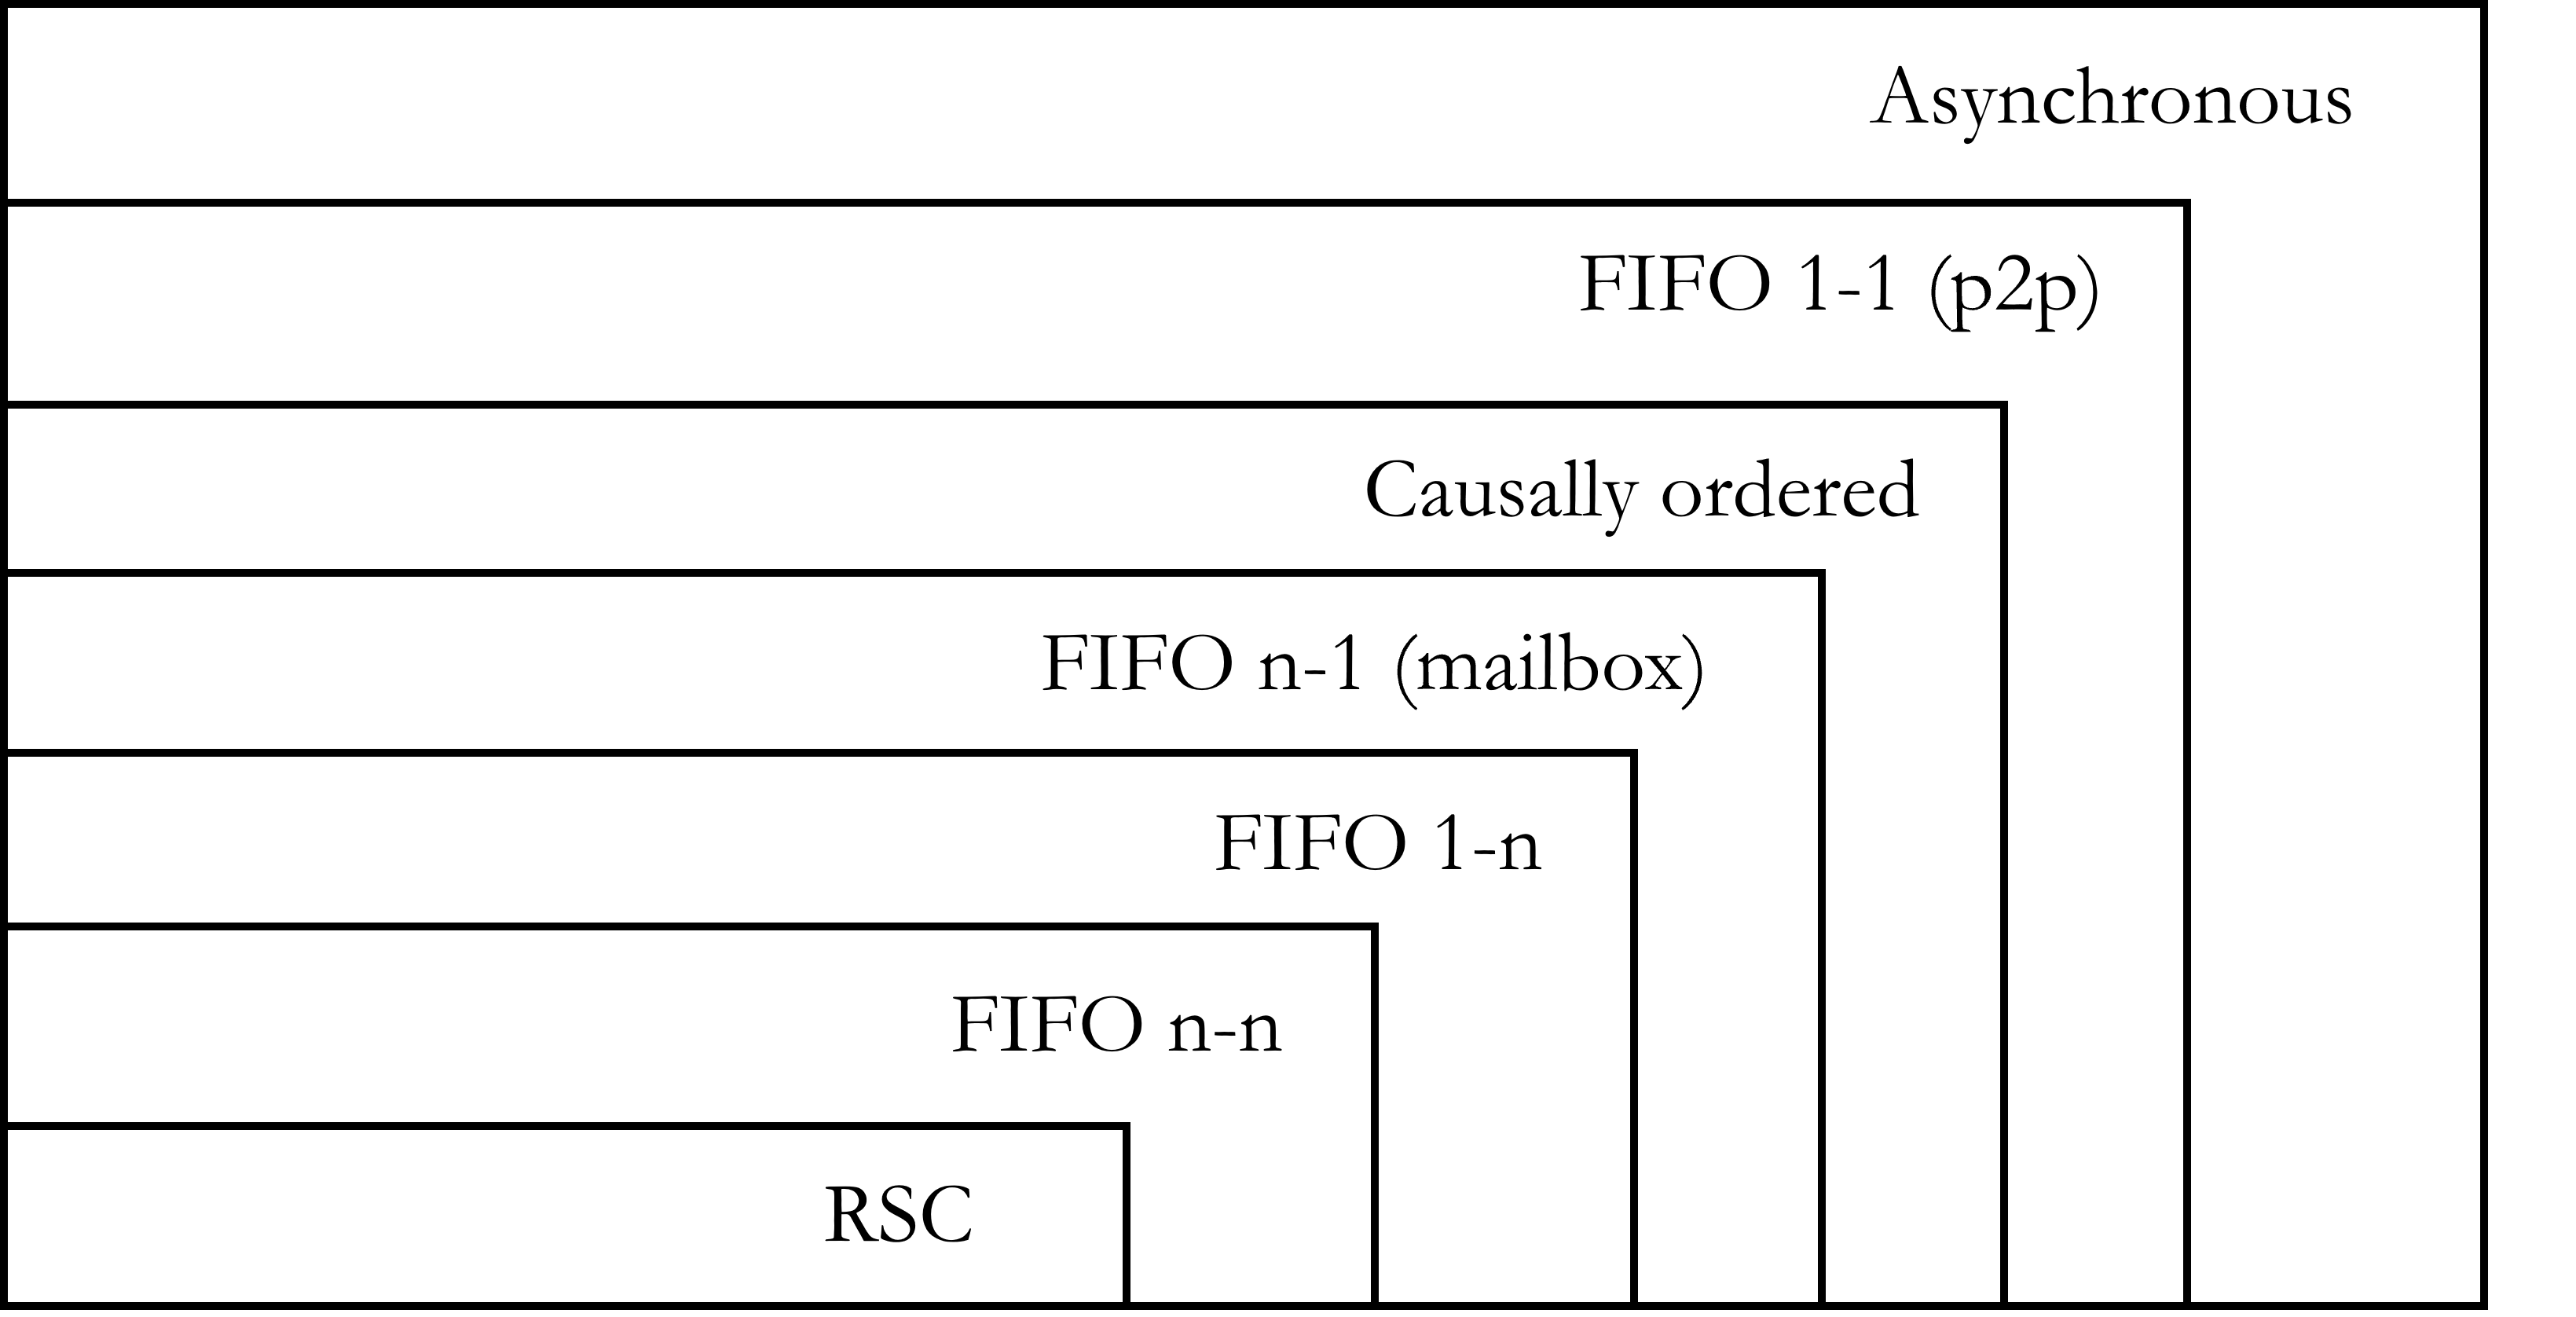
\includegraphics[width=8cm]{msc_hierarchy}
	\caption{The hierarchy of MSC classes.}
	\label{fig:msc_hierarchy}
\end{figure}

\subsection{Monadic Second-Order Logic}

The set of MSO formulas over (asynchronous) MSCs (over $\Procs$ and $\Msg$) is given by the grammar
$
\phi ::= true \mid x \procrel y \mid x \lhd y \mid \lambda(x) = a \mid x = y \mid x \in X \mid \exists x.\phi \mid \exists X.\phi \mid \phi \vee \phi \mid \neg \phi
$,
where $a \in \Act$, $x$ and $y$ are first-order variables, interpreted as
events of an MSC, and $X$ is a second-order variable, interpreted
as a set of events. We assume that we have an infinite supply of variables,
and we use common abbreviations such as $\wedge$, $\Rightarrow$, $\forall$, etc.
The satisfaction relation is defined in the standard way and self-explanatory.
For example, the formula $\neg\exists x.(\bigvee_{a \in \sAct} \lambda(x) = a \;\wedge\; \neg \mathit{matched}(x))$
with $\mathit{matched}(x) = \exists y.x \lhd y$
says that there are no unmatched send events.
It is not satisfied by  MSC $\mscweakuniver$
of Fig.~\ref{fig:msc_weak_univer},
as message $\msg_1$ is not received,
but by $\mscstrongexist$ from Fig.~\ref{fig:msc_strong_exist}.

Given a sentence $\phi$, i.e., a formula without free variables,
we let $L(\phi)$ denote the set of MSCs that satisfy $\phi$. Since we have defined the set of MSO formulas over asynchronous MSCs, the formula $\asformula = true$ clearly describes the set of asynchronous MSCs, i.e. $L(\asformula) = \asMSCs$. It is worth mentioning that the (reflexive) transitive closure of a binary relation defined by an MSO formula\footnote{See Section~\ref{sec:mso_extra} for details.} with free variables $x$ and $y$, such as $x \procrel y$, is MSO-definable so that the logic can freely use formulas of the form $x \procrel^+ y$, $x \procrel^* y$ or $x \le y$ (where $\le$ is interpreted as $\le_\msc$ for the given MSC $\msc$).

\paragraph*{Peer-to-peer MSCs}
	The set of \pp MSCs is MSO-definable as
	\[
		\ppformula = \neg \exists s.\exists s'. \left(
		\bigvee_{\substack{p \in \Procs, q \in \Procs}}\;
		\bigvee_{\substack{a,b \in \pqsAct{p}{q}}}\hspace{-1em}
		(\lambda(s) = a \;\wedge\; \lambda(s') = b) \;\wedge\; s \procrel^+ s' \;\wedge\;
		(\psi_1 \vee \psi_2 ) 	
		\right)
	\]
	where $\psi_1$ and $\psi_2$ are
	\[
		\psi_1 = \exists r.\exists r'.\left(
		\begin{array}{ll}
			s \lhd r & \wedge\\
			s' \lhd r' & \wedge\\
			r' \procrel^+ r &
		\end{array} 
		\right) \quad \quad
		\psi_2 = (\neg \mathit{matched}(s) \wedge \mathit{matched}(s'))
		\]
		\[
		matched(x) = \exists y. x \lhd y
	\]

The property $\ppformula$ says that there cannot be two matched send events $s$ and $s'$, with the same sender and receiver, such that either
\begin{enumerate*}[label={(\roman*)}]
	\item $s \procrel^+ s'$ and their receipts happen in the reverse order, or
	\item $s$ is unmatched and $s'$ is matched.
\end{enumerate*}
In other words, it ensures that channels operate in FIFO mode, where an unmatched messages blocks the receipt of all the subsequent messages on that channel.
The set $\ppMSCs$ is therefore MSO-definable as $\ppMSCs=L(\ppformula)$.

\paragraph*{Causally ordered MSCs}
Given an MSC $\msc$, it is causally ordered if and only if it satisfies the MSO formula
\[
	\coformula = \neg \exists s.\exists s'. \left(
	\bigvee_{\substack{q \in \Procs}}\;
	\bigvee_{\substack{a,b \in \pqsAct{\plh}{q}}}\hspace{-1em}
	(\lambda(s) = a \;\wedge\; \lambda(s') = b) \;\wedge\; s \le_\msc s' \;\wedge\;
	(\psi_1 \vee \psi_2 ) 	
	\right)
\]
where $\psi_1$ and $\psi_2$ are the same formulas used for \pp.

The property $\coformula$ says that there cannot be two send events $s$ and $s'$, with the same recipient, such that $s \le_\msc s'$ and either
\begin{enumerate*}[label={(\roman*)}]
	\item their corresponding receive events $r$ and $r'$ happen in the opposite order, i.e. $r' \procrel^+ r$, or
	\item $s$ is unmatched and $s'$ is matched.
\end{enumerate*}
The set $\coMSCs$ of causally ordered MSCs is therefore MSO-definable as $\coMSCs=L(\coformula)$.

\paragraph*{Mailbox MSCs}

Given an MSC $\msc$, it is a mailbox MSC if and only if it satisfies the MSO formula
\[
	\mbformula = \ppformula \;\wedge\; \neg \exists x.\exists y.(\neg (x = y) \wedge x \preceq_\msc y \wedge y \preceq_\msc x)
\]
The set $\mbMSCs$ of mailbox MSCs is therefore MSO-definable as $\mbMSCs=L(\mbformula)$.
\davide{This does not match my definition of mailbox MSC, should I also give the alternative definition (the one in the concur paper) or rewrite everything according to my definition? Give both definitions and prove that they are equivalent}

\paragraph*{$\onen$ MSCs}

Following Definition~\ref{def:one_n_alt}, an MSC $\msc$ is a $\onen$ MSC if and only if it satisfies the MSO formula
\[
	\onenformula = \neg \exists x.\exists y.(\neg (x = y) \wedge x \lessdot_\msc y \wedge y \lessdot_\msc x)
\]
Recall that $\lessdot_\msc$ is the union of the MSO-definable relations $\procrel$, $\lhd$, and $\onenrel_\msc$. In particular, we can define $x \onenrel_\msc y$ as 
\[
x \onenrel_\msc y =
\begin{array}{rl}
& \left(
	\bigvee_{\substack{p \in \Procs\\a,b \in \psAct{p}}}\hspace{-1em}
	(\lambda(x) = a \;\wedge\; \lambda(y) = b)
	\;\wedge\; \mathit{matched}(x) \;\wedge\; \neg \mathit{matched}(y)
\right) \;\vee\\
& \left(
	\bigvee_{\substack{p \in \Procs\\a,b \in \prAct{p}}}\hspace{-1em}
	(\lambda(x) = a \;\wedge\; \lambda(y) = b)
	\;\wedge\; 
	\exists x'.\exists y'. (x' \lhd x \;\wedge\; y' \lhd y \;\wedge\; x' \procrel^+ y')
\right)\\
\end{array}
\]
The MSO formula for $x \onenrel_\msc y$ closely follows Definition~\ref{def:one_n_alt}. The set $\onenMSCs$ of $\onen$ MSCs is therefore MSO-definable as $\onenMSCs=L(\onenformula)$.

\paragraph*{$\nn$ MSCs}

Following Definition~\ref{def:n_n_alt}, an MSC $\msc$ is a $\nn$ MSC if and only if it satisfies the MSO formula
\[
	\nnformula = \neg \exists x.\exists y.(\neg (x = y) \wedge x \bowtie_\msc y \wedge y \bowtie_\msc x)
\]
In particular, we can define $x \bowtie_\msc y$ as
\[
	x \bowtie_\msc y =
	\begin{array}{rl}
	& \left(
		\bigvee_{\substack{a,b \in \psAct{\plh}}}
		(\lambda(x) = a \;\wedge\; \lambda(y) = b)
		\;\wedge\; \mathit{matched}(x) \;\wedge\; \neg \mathit{matched}(y)
	\right) \;\vee\\
	& (x \nnrel_\msc y) \quad \vee \quad \psi_3 \quad \vee \quad \psi_4\\
	\end{array}
\]

\noindent where $\psi_3$ and $\psi_4$ are defined as 
\[
	\psi_3 =
	\begin{array}{rl}
		& \bigvee_{\substack{a,b \in \prAct{\plh}}}
		  (\lambda(x) = a \;\wedge\; \lambda(y) = b)
		  \;\wedge\; \\
		& \exists x'.\exists y'.(x' \lhd x \;\wedge\; y' \lhd y) \;\wedge\; (x' \nnrel_\msc y') \;\wedge\; \neg(x \nnrel_\msc y)\\
	\end{array}
\]
\[
	\psi_4 =
	\begin{array}{rl}
		& \bigvee_{\substack{a,b \in \psAct{\plh}}}
		  (\lambda(x) = a \;\wedge\; \lambda(y) = b)
		  \;\wedge\; \\
		& \exists x'.\exists y'.(x \lhd x' \;\wedge\; y \lhd y') \;\wedge\; (x' \nnrel_\msc y') \;\wedge\; \neg(x \nnrel_\msc y)\\
	\end{array}
\]

The MSO formula for $x \nnrel_\msc y$ closely follows Definition~\ref{def:n_n_alt}. The set $\nnMSCs$ of $\nn$ MSCs is therefore MSO-definable as $\nnMSCs=L(\nnformula)$.

\paragraph*{$\rsc$ MSCs}

Following Definition~\ref{def:rsc_alt}, an MSC $\msc$ is a $\rsc$ MSC if and only if it satisfies the MSO formula
\[
\Phi_{\rsc} = \neg \exists s_1.\exists s_2. s_1 \varpropto s_2 \;\wedge\; s_2 \varpropto^\ast s_1
\]
\noindent where $\varpropto$ is defined as
\[
s_1 \varpropto s_2 = 
\bigvee_{\substack{e \in \sAct}}(\lambda(s_1) = e) \;\wedge\;
s_1 \neq s_2 \;\wedge\; 
\exists r_2. (s_1 < r_2 \;\wedge\; s_2 \lhd r_2)
\]
% \davidequestion{The following formula should be wrong... I cannot use $n$ in an MSO formula}
% \[
% 	\rscformula = 
% 	\begin{array}{rl}
% 		& \forall x.\left(\bigvee_{a \in \psAct{\plh}} \lambda(x) = a \;\implies\; \mathit{matched}(x)\right) \;\wedge\; \\
% 		& \neg \left( 
% 			\bigvee_{k=1}^n \left(
% 			\exists s_1 \cdots s_k. \exists r_1 \cdots r_k. 
% 			\bigwedge_{i=1}^k (s_i \lhd r_i \;\wedge\; s_i \le_\msc r_{(i+1)\%k})
% 		\right)
% 		\right)\\
% 	\end{array}
% \]
% where $n$ is the total number of messages. The formula checks that there are no unmatched send events and that in the conflict graph there is no cycle, of any length, whose edges are all SR.